% Options for packages loaded elsewhere
% Options for packages loaded elsewhere
\PassOptionsToPackage{unicode}{hyperref}
\PassOptionsToPackage{hyphens}{url}
\PassOptionsToPackage{dvipsnames,svgnames,x11names}{xcolor}
%
\documentclass[
  letterpaper,
  DIV=11,
  numbers=noendperiod]{scrartcl}
\usepackage{xcolor}
\usepackage{amsmath,amssymb}
\setcounter{secnumdepth}{-\maxdimen} % remove section numbering
\usepackage{iftex}
\ifPDFTeX
  \usepackage[T1]{fontenc}
  \usepackage[utf8]{inputenc}
  \usepackage{textcomp} % provide euro and other symbols
\else % if luatex or xetex
  \usepackage{unicode-math} % this also loads fontspec
  \defaultfontfeatures{Scale=MatchLowercase}
  \defaultfontfeatures[\rmfamily]{Ligatures=TeX,Scale=1}
\fi
\usepackage{lmodern}
\ifPDFTeX\else
  % xetex/luatex font selection
\fi
% Use upquote if available, for straight quotes in verbatim environments
\IfFileExists{upquote.sty}{\usepackage{upquote}}{}
\IfFileExists{microtype.sty}{% use microtype if available
  \usepackage[]{microtype}
  \UseMicrotypeSet[protrusion]{basicmath} % disable protrusion for tt fonts
}{}
\makeatletter
\@ifundefined{KOMAClassName}{% if non-KOMA class
  \IfFileExists{parskip.sty}{%
    \usepackage{parskip}
  }{% else
    \setlength{\parindent}{0pt}
    \setlength{\parskip}{6pt plus 2pt minus 1pt}}
}{% if KOMA class
  \KOMAoptions{parskip=half}}
\makeatother
% Make \paragraph and \subparagraph free-standing
\makeatletter
\ifx\paragraph\undefined\else
  \let\oldparagraph\paragraph
  \renewcommand{\paragraph}{
    \@ifstar
      \xxxParagraphStar
      \xxxParagraphNoStar
  }
  \newcommand{\xxxParagraphStar}[1]{\oldparagraph*{#1}\mbox{}}
  \newcommand{\xxxParagraphNoStar}[1]{\oldparagraph{#1}\mbox{}}
\fi
\ifx\subparagraph\undefined\else
  \let\oldsubparagraph\subparagraph
  \renewcommand{\subparagraph}{
    \@ifstar
      \xxxSubParagraphStar
      \xxxSubParagraphNoStar
  }
  \newcommand{\xxxSubParagraphStar}[1]{\oldsubparagraph*{#1}\mbox{}}
  \newcommand{\xxxSubParagraphNoStar}[1]{\oldsubparagraph{#1}\mbox{}}
\fi
\makeatother


\usepackage{longtable,booktabs,array}
\usepackage{calc} % for calculating minipage widths
% Correct order of tables after \paragraph or \subparagraph
\usepackage{etoolbox}
\makeatletter
\patchcmd\longtable{\par}{\if@noskipsec\mbox{}\fi\par}{}{}
\makeatother
% Allow footnotes in longtable head/foot
\IfFileExists{footnotehyper.sty}{\usepackage{footnotehyper}}{\usepackage{footnote}}
\makesavenoteenv{longtable}
\usepackage{graphicx}
\makeatletter
\newsavebox\pandoc@box
\newcommand*\pandocbounded[1]{% scales image to fit in text height/width
  \sbox\pandoc@box{#1}%
  \Gscale@div\@tempa{\textheight}{\dimexpr\ht\pandoc@box+\dp\pandoc@box\relax}%
  \Gscale@div\@tempb{\linewidth}{\wd\pandoc@box}%
  \ifdim\@tempb\p@<\@tempa\p@\let\@tempa\@tempb\fi% select the smaller of both
  \ifdim\@tempa\p@<\p@\scalebox{\@tempa}{\usebox\pandoc@box}%
  \else\usebox{\pandoc@box}%
  \fi%
}
% Set default figure placement to htbp
\def\fps@figure{htbp}
\makeatother


% definitions for citeproc citations
\NewDocumentCommand\citeproctext{}{}
\NewDocumentCommand\citeproc{mm}{%
  \begingroup\def\citeproctext{#2}\cite{#1}\endgroup}
\makeatletter
 % allow citations to break across lines
 \let\@cite@ofmt\@firstofone
 % avoid brackets around text for \cite:
 \def\@biblabel#1{}
 \def\@cite#1#2{{#1\if@tempswa , #2\fi}}
\makeatother
\newlength{\cslhangindent}
\setlength{\cslhangindent}{1.5em}
\newlength{\csllabelwidth}
\setlength{\csllabelwidth}{3em}
\newenvironment{CSLReferences}[2] % #1 hanging-indent, #2 entry-spacing
 {\begin{list}{}{%
  \setlength{\itemindent}{0pt}
  \setlength{\leftmargin}{0pt}
  \setlength{\parsep}{0pt}
  % turn on hanging indent if param 1 is 1
  \ifodd #1
   \setlength{\leftmargin}{\cslhangindent}
   \setlength{\itemindent}{-1\cslhangindent}
  \fi
  % set entry spacing
  \setlength{\itemsep}{#2\baselineskip}}}
 {\end{list}}
\usepackage{calc}
\newcommand{\CSLBlock}[1]{\hfill\break\parbox[t]{\linewidth}{\strut\ignorespaces#1\strut}}
\newcommand{\CSLLeftMargin}[1]{\parbox[t]{\csllabelwidth}{\strut#1\strut}}
\newcommand{\CSLRightInline}[1]{\parbox[t]{\linewidth - \csllabelwidth}{\strut#1\strut}}
\newcommand{\CSLIndent}[1]{\hspace{\cslhangindent}#1}



\setlength{\emergencystretch}{3em} % prevent overfull lines

\providecommand{\tightlist}{%
  \setlength{\itemsep}{0pt}\setlength{\parskip}{0pt}}



 


\KOMAoption{captions}{tableheading}
\makeatletter
\@ifpackageloaded{caption}{}{\usepackage{caption}}
\AtBeginDocument{%
\ifdefined\contentsname
  \renewcommand*\contentsname{Table of contents}
\else
  \newcommand\contentsname{Table of contents}
\fi
\ifdefined\listfigurename
  \renewcommand*\listfigurename{List of Figures}
\else
  \newcommand\listfigurename{List of Figures}
\fi
\ifdefined\listtablename
  \renewcommand*\listtablename{List of Tables}
\else
  \newcommand\listtablename{List of Tables}
\fi
\ifdefined\figurename
  \renewcommand*\figurename{Figure}
\else
  \newcommand\figurename{Figure}
\fi
\ifdefined\tablename
  \renewcommand*\tablename{Table}
\else
  \newcommand\tablename{Table}
\fi
}
\@ifpackageloaded{float}{}{\usepackage{float}}
\floatstyle{ruled}
\@ifundefined{c@chapter}{\newfloat{codelisting}{h}{lop}}{\newfloat{codelisting}{h}{lop}[chapter]}
\floatname{codelisting}{Listing}
\newcommand*\listoflistings{\listof{codelisting}{List of Listings}}
\makeatother
\makeatletter
\makeatother
\makeatletter
\@ifpackageloaded{caption}{}{\usepackage{caption}}
\@ifpackageloaded{subcaption}{}{\usepackage{subcaption}}
\makeatother
\usepackage{bookmark}
\IfFileExists{xurl.sty}{\usepackage{xurl}}{} % add URL line breaks if available
\urlstyle{same}
\hypersetup{
  pdftitle={Predicting Daily Land Average Temperature},
  pdfauthor={Molly Kessler, Daisy Zhou, Ojasv Issar, Jacob Cann},
  colorlinks=true,
  linkcolor={blue},
  filecolor={Maroon},
  citecolor={Blue},
  urlcolor={Blue},
  pdfcreator={LaTeX via pandoc}}


\title{Predicting Daily Land Average Temperature}
\author{Molly Kessler, Daisy Zhou, Ojasv Issar, Jacob Cann}
\date{}
\begin{document}
\maketitle

\renewcommand*\contentsname{Table of contents}
{
\hypersetup{linkcolor=}
\setcounter{tocdepth}{3}
\tableofcontents
}

\section{Summary}\label{summary}

This project analyzes global daily average land-surface temperature
measurements collected by Berkeley Earth from 1880--2022. In the
following analysis, dataset is cleaned and preprocessed, explored
through EDA, and modeled to predict future temperature trends using this
historical data. After evaluating three regression approaches, Linear
Regression, Random Forest, and Support Vector Regression (SVR),the SVR
model performed best and was used to forecast the land average
temperature for the year 2030.

\section{Introduction}\label{introduction}

Understanding long-term changes in global land temperature is critical
for studying climate change. Daily temperature anomaly data collected
over more than 140 years provide an opportunity to model how
temperatures have shifted, identify long-term patterns, and forecast
future warming.

In this report, we talk both about the actual temperature as well as the
temperature anomaly. Temperature anomaly refers to deviation from a
baseline climatological temperature. In this study, the baseline is
8.59°C, representing the January 1951--December 1980 global land-average
temperature.

In this project, we will be answering the research question:

What do we expect the global land-average temperature of the Earth to be
in 2030, based on the trends from the years 1880 to 2012.

\subsection{Dataset}\label{dataset}

The data set for this project was published by Berkeley Earth under a
Creative Commons BY-NC 4.0 International license, free for
non-commercial use, and accessed by our team compliant with the
conditions in this license on November 18, 2025. The raw data can be
found at the
\href{https://berkeley-earth-temperature.s3.us-west-1.amazonaws.com/Global/Complete_TAVG_daily.txt}{Berkeley
Earth Temperature site} (Berkeley Earth, n.d.).

The data set contains 5 columns with time series information, and one
column representing the temperature difference relative to the average
temperature between January 1951 and December 1980, which they
calculated as 8.59 +/- 0.05. For our analysis, we preprocessed the data
to get the raw temperature readings back by adding 8.59 to each entry in
the Anomaly column. All temperatures are in Celsius.

\section{Methods and Results}\label{methods-and-results}

The Python programming language (Van Rossum and Drake 2009) and the
following Python packages were used to perform the analysis: pandas
(McKinney 2010), altair (VanderPlas 2018), click (Team 2020), as well as
Quarto (Allaire et al. 2022). \textbf{ADD matplotlib and pandera,
sklearn, python etc.}

\subsection{Pandera Schema for Daily Temperature Data
Validation}\label{pandera-schema-for-daily-temperature-data-validation}

This Pandera schema defines the expected structure and quality checks
for the daily temperature dataset. It enforces correct column names,
validates data types (e.g., integers for dates, floats for temperature
values), ensures month names follow the expected categories, checks that
values fall within reasonable ranges (year, month, day, day-of-year),
and confirms that no duplicate rows are present. Setting
\texttt{strict=True} prevents unexpected columns from slipping in, and
\texttt{coerce=True} allows Pandera to automatically convert compatible
types when possible.

** ADD THE IN LINE CITATIONS HERE **

The allowable limits for outliers on the average temperature anomaly
dataset relative to the average baseline (estimated Jan.~1951 -
Dec.~1980 absolute temperature with reported 95\% confidence bounds),
were naturally set as the minimum and maximum measurements of the
baseline itself, or in other words the minimum and maximum temperature
anomalies observed. These are reasonable limits for the averaged values
because you would not expect the averaged values to be anywhere near the
absolute minimum and maximum measurements, and if they are these
examples should be examined more carefully (raising a validation warning
or viewing the validation error log). Because the baseline, temperature
in Celsius and temperature anomaly are all related, bounds can be set on
the anomaly target or temperature target interchangeably by adding or
subtracting the average baseline (8.59). The resulting average anomaly
limits were -5.64 and 5.81, which were compared to external sources to
ensure validity. The sources cited above, (which use the same 1951-1980
baseline for average temperature anomaly) demonstrate that a deviation
of temperature anomaly by more than 5 degrees Celsius from the baseline
is extremely rare, and only observed for certain monthly averages of
anomaly temperature taken across specific regions: ``It was unusually
warm in the Southeast U.S. and Greenland in December, the monthly
average anomaly exceeding +5°C (+9°F) (Fig. 3)''{[}5{]}. Since our
dataset involves average temperature anomalies globally, an anomaly this
large in magnitude entering the training dataset should be flagged in
the validation stage, examined further and potentially discarded.

\subsection{Load the Data}\label{load-the-data}

Load the daily land-surface average anomaly data provided by Berkeley
Earth collected from 1880 to 2022.

\subsection{File type check}\label{file-type-check}

\subsection{Data Pre-Processing}\label{data-pre-processing}

\subsection{Validating The Full
Dataframe}\label{validating-the-full-dataframe}

\begin{verbatim}
✓ Data validation passed
\end{verbatim}

\subsubsection{Data Splitting}\label{data-splitting}

\begin{longtable}[]{@{}llllllll@{}}
\toprule\noalign{}
& Year & Month & Day & Day of Year & Anomaly & Temperature &
Month\_Name \\
\midrule\noalign{}
\endhead
\bottomrule\noalign{}
\endlastfoot
0 & 1880 & 1 & 1 & 1 & -0.692 & 7.898 & January \\
1 & 1880 & 1 & 2 & 2 & -0.592 & 7.998 & January \\
2 & 1880 & 1 & 3 & 3 & -0.673 & 7.917 & January \\
3 & 1880 & 1 & 4 & 4 & -0.615 & 7.975 & January \\
4 & 1880 & 1 & 5 & 5 & -0.681 & 7.909 & January \\
... & ... & ... & ... & ... & ... & ... & ... \\
48573 & 2012 & 12 & 27 & 361 & 0.134 & 8.724 & December \\
48574 & 2012 & 12 & 28 & 362 & 0.371 & 8.961 & December \\
48575 & 2012 & 12 & 29 & 363 & 0.532 & 9.122 & December \\
48576 & 2012 & 12 & 30 & 364 & 0.594 & 9.184 & December \\
48577 & 2012 & 12 & 31 & 365 & 0.631 & 9.221 & December \\
\end{longtable}

\subsection{Validating The Training
Dataframe}\label{validating-the-training-dataframe}

\begin{verbatim}
<VegaLite 5 object>

If you see this message, it means the renderer has not been properly enabled
for the frontend that you are using. For more information, see
https://altair-viz.github.io/user_guide/display_frontends.html#troubleshooting
\end{verbatim}

We can see from the histogram plots of the target (Anomaly untransformed
and Temperature when transformed) that the distribution of the target is
very slightly right-skewed, but is almost symmetric and fairly
bell-shaped. It make sense that the majority of the distribution is
close to normally distributed as temperature increase has accelerated in
recent years and was less prevalent the further you go back in time. We
would expect the distribution to be right-skewed since the accepted
hypothesis of average global temperature is that it is increasing and
accelerating in recent years relative to when the collection of this
data first began, and this would cause more of the density of the
anomaly and temperature distributions to be to the left of the mean.

\begin{verbatim}
✓ Data validation passed
\end{verbatim}

\begin{verbatim}
<VegaLite 5 object>

If you see this message, it means the renderer has not been properly enabled
for the frontend that you are using. For more information, see
https://altair-viz.github.io/user_guide/display_frontends.html#troubleshooting
\end{verbatim}

\subsubsection{Correlation Checks Using
DEEPCHECKS}\label{correlation-checks-using-deepchecks}

The validation checks are set to raise warnings if there are unexpected
anomalous correlations among features or between features and the
target. Any warnings raise should be examined carefully in conjunction
with the correlation plot above. Some columns have been intentionally
dropped for this training dataset correlation analysis because they are
known to have a correlation that makes sense and does not affect the
analysis. For example (and shown clearly below), Month and Day of Year
will be very strongly correlated as they measure the same thing but in
different intervals. Additionally, Anomaly and Temperature will have a
correlation of 1 since they are transformations of each other by
addition of a constant. Anomaly and Temperature are expected to be
correlated with the Year as this relationship is well-known and part of
the reason reasonable forecasts can be made by the model in this
analysis.

\begin{verbatim}
DataTransformerRegistry.enable('default')
\end{verbatim}

\begin{verbatim}
<VegaLite 5 object>

If you see this message, it means the renderer has not been properly enabled
for the frontend that you are using. For more information, see
https://altair-viz.github.io/user_guide/display_frontends.html#troubleshooting
\end{verbatim}

\subsection{Exploratory Data Analysis
(EDA)}\label{exploratory-data-analysis-eda}

The goal of this EDA is to determine what type of predictive model will
be the best fit for the data. A suitable regression method is to
explored, as the target (global average land temperature) is continuous.
After preprocessing the dataset, no presence of null values were found
requiring attention. In order to make the Month\_Name (converting from
Month) feature more readable during EDA, the feature was converted to an
ordinal feature, with Jan as the first in the order and December as the
last in the order. Monthly trends in the data were considered over the
years, however overall trends were found irrespective of the month the
data was collected in. A cutoff year was decided for splitting the data
into test and training data sets (see code below), and EDA was carried
out on only the training portion of the data set to avoid violating the
golden rule and double dipping. A randomized test split was not
implemented as the model is desired for predicting temperatures in the
future, so test data taken from the latest measurements represents the
best evaluation of the regression model. Once the dataset was split, EDA
was performed with several visualization strategies, the most
informative of which are presented below. Discussions of the findings
and rationale are found below as well.

\begin{verbatim}
<class 'pandas.core.frame.DataFrame'>
Index: 48578 entries, 0 to 48577
Data columns (total 7 columns):
 #   Column       Non-Null Count  Dtype  
---  ------       --------------  -----  
 0   Year         48578 non-null  int64  
 1   Month        48578 non-null  int64  
 2   Day          48578 non-null  int64  
 3   Day of Year  48578 non-null  int64  
 4   Anomaly      48578 non-null  float64
 5   Temperature  48578 non-null  float64
 6   Month_Name   48578 non-null  object 
dtypes: float64(2), int64(4), object(1)
memory usage: 3.0+ MB
\end{verbatim}

\begin{longtable}[]{@{}lllllll@{}}
\toprule\noalign{}
& Year & Month & Day & Day of Year & Anomaly & Temperature \\
\midrule\noalign{}
\endhead
\bottomrule\noalign{}
\endlastfoot
count & 48578.000000 & 48578.000000 & 48578.000000 & 48578.000000 &
48578.000000 & 48578.000000 \\
mean & 1946.000947 & 6.522953 & 15.729569 & 183.000000 & 0.016194 &
8.606194 \\
std & 38.393532 & 3.448732 & 8.800154 & 105.331318 & 0.607513 &
0.607513 \\
min & 1880.000000 & 1.000000 & 1.000000 & 1.000000 & -2.728000 &
5.862000 \\
25\% & 1913.000000 & 4.000000 & 8.000000 & 92.000000 & -0.367000 &
8.223000 \\
50\% & 1946.000000 & 7.000000 & 16.000000 & 183.000000 & -0.034000 &
8.556000 \\
75\% & 1979.000000 & 10.000000 & 23.000000 & 274.000000 & 0.372750 &
8.962750 \\
max & 2012.000000 & 12.000000 & 31.000000 & 365.000000 & 2.552000 &
11.142000 \\
\end{longtable}

\begin{verbatim}
Year           False
Month          False
Day            False
Day of Year    False
Anomaly        False
Temperature    False
Month_Name     False
dtype: bool
\end{verbatim}

Due to the many measurements that occur in each year (contributing to
plotting noise), the mean of the temperatures for each group of
measurements taken in a year were plotted in addition to the raw data
points of temperature over time. A general trend of increasing
temperature over time with local fluctuations can be observed below.

\begin{verbatim}
<VegaLite 5 object>

If you see this message, it means the renderer has not been properly enabled
for the frontend that you are using. For more information, see
https://altair-viz.github.io/user_guide/display_frontends.html#troubleshooting
\end{verbatim}

Using the mean data points by year, a linear regression model was fit to
the training data to assess the viability of this approach in
prediction. The linear regression fit can be seen to follow the overall
trend, but misses information about local fluctuations, seen by the
points above and below the line. A linear model has potential to
generalize for unseen year examples but may be too simple for this
analysis and will not be precise in its predictions for every year. A
5-year rolling average was also explored, due to its ability to adapt
the curve more effectively to local fluctuations. However, a model of
this type may not extrapolate well for unseen examples to predict future
temperatures.

\begin{verbatim}
<VegaLite 5 object>

If you see this message, it means the renderer has not been properly enabled
for the frontend that you are using. For more information, see
https://altair-viz.github.io/user_guide/display_frontends.html#troubleshooting
\end{verbatim}

In order to check if the global average daily temperature over time was
affected by seasonal phenomena, the annual means of these temperature
measurements were analyzed by each month separated. It can be seen from
the facet plot below that regardless of the season global daily average
land temperature measurements are increasing non-trivially over time.

\begin{verbatim}
<VegaLite 5 object>

If you see this message, it means the renderer has not been properly enabled
for the frontend that you are using. For more information, see
https://altair-viz.github.io/user_guide/display_frontends.html#troubleshooting
\end{verbatim}

Finally, the distribution of the training data for temperature with
respect to distinct year separated in by approximately 60 years were
evaluated for distinct eras in the density plot below. The last year in
the training data set (the cutoff year defined above) can be seen as
significantly shifted to the right, indicating the increase in global
daily average land temperature across time. Three distinct peaks in the
density plot below reinforces the hypothesis that even when account for
the variance in temperature due to local fluctuations, the overall trend
of global temperature increasing over time remains.

\begin{verbatim}
<VegaLite 5 object>

If you see this message, it means the renderer has not been properly enabled
for the frontend that you are using. For more information, see
https://altair-viz.github.io/user_guide/display_frontends.html#troubleshooting
\end{verbatim}

\subsection{Machine Learning
Modelling}\label{machine-learning-modelling}

Here we convert daily climate data into yearly averages by creating a
proper datetime index, resampling the anomaly values to annual means,
and preparing the data for modeling by extracting the numerical year and
separating it into feature (X) and target (y) arrays. Yearly averages
smooth out short-term noise and make long-term climate trends easier to
model, and using the year as the feature allows the machine-learning
models to learn how temperature anomalies evolve over time.

We split the data into a training set (years up to 2012) and a test set
(years after 2012) by creating boolean masks based on the chosen split
year. It then uses those masks to separate the feature matrix and target
values into training and testing subsets. By training on earlier years
and testing on later years, we evaluate how well the model predicts
future climate patterns rather than just fitting past data. A good model
should perform well on the test set, meaning it can generalize to years
it has never seen before.

Three different machine-learning models are defined which are Linear
Regression, Random Forest, and a Support Vector Regressor (SVR) with
scaling---so we can compare how well each one predicts yearly
temperature anomalies. Each model captures patterns differently, ranging
from simple linear trends to more flexible non-linear relationships.

We train each defined model on the training data, predicts anomalies for
the test years, and calculates key evaluation metrics (RMSE, MAE, R²) to
measure prediction accuracy. The results are stored in a table for easy
comparison of model performance.

\begin{verbatim}

Model Performance on Test Set:

                       RMSE       MAE         R2
Linear Regression  0.539126  0.521939 -11.652955
Random Forest      0.350576  0.316120  -4.350267
SVR                0.143855  0.119263   0.099127
\end{verbatim}

Lower RMSE and MAE values indicate more accurate predictions, while a
higher (positive) R² shows the model explains more variance in the data.
From the table, SVR has the lowest errors and a positive R², making it
the best model to use for forecasting.

\begin{verbatim}

Best model: SVR
\end{verbatim}

We use the selected best model (SVR) to predict the temperature anomaly
for the year 2030 and then adds it to the baseline temperature to
estimate the actual land-average temperature.

\begin{verbatim}

Predicted anomaly for 2030: 1.9646 °C
Predicted land-average temperature for 2030: 10.5546 °C
\end{verbatim}

\textbf{ADD THE INLINE CODE VARIABLE REFERENCES FOR THIS}

The predicted anomaly of \textbf{≈1.97\,°C} indicates that 2030 is
expected to be nearly 2\,°C warmer than the baseline period. Adding this
to the baseline gives a land-average temperature of \textbf{≈10.56\,°C},
showing a continuation of the observed warming trend.

\pandocbounded{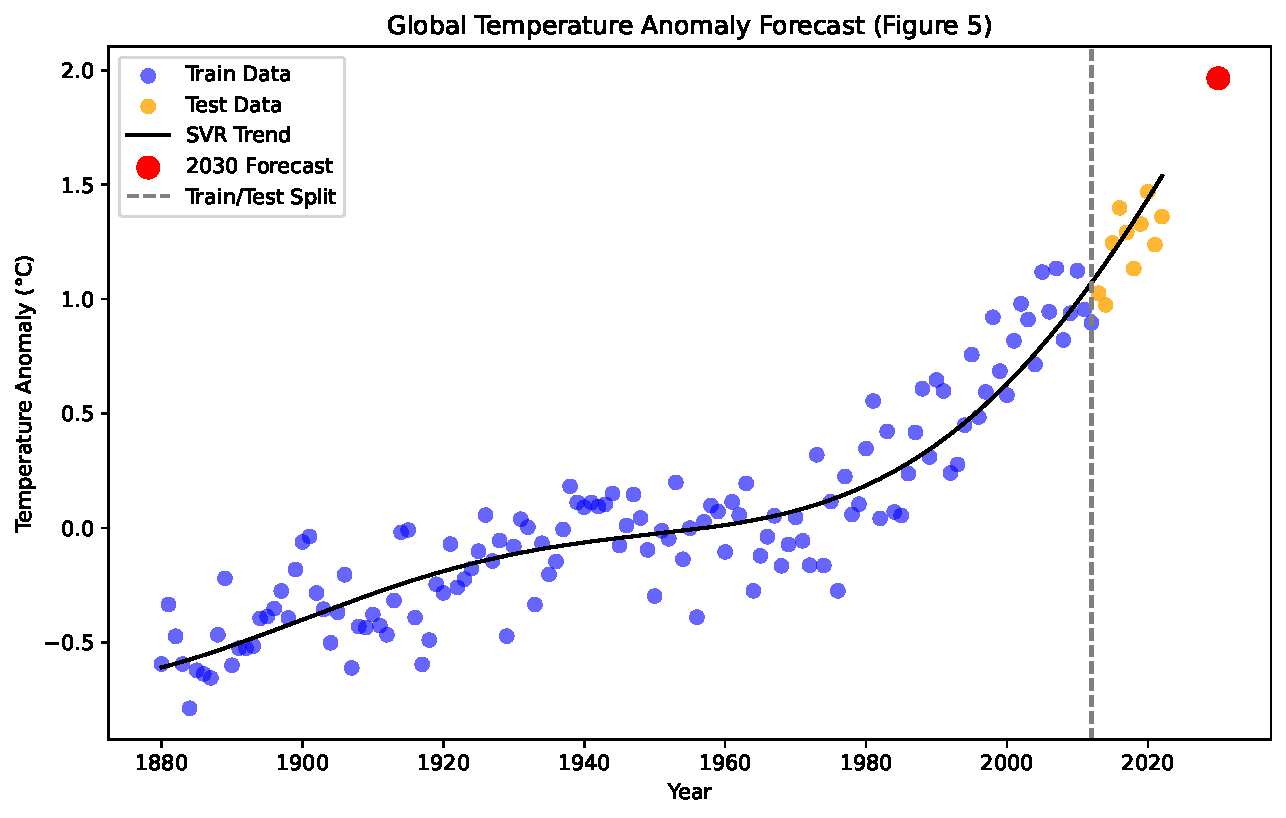
\includegraphics[keepaspectratio]{global_daily_land_temperature_prediction_files/figure-pdf/cell-32-output-1.pdf}}

The plot shows the historical anomalies, with training data in blue and
test data in orange, allowing us to visually compare the model's
predictions against unseen years. The black trend line from the SVR
model captures the warming pattern, while the red point highlights the
2030 forecast, illustrating the expected continuation of the temperature
rise.

The trend line closely follows historical data, test points are
reasonably well-predicted, and the red forecast indicates that
temperature anomalies are expected to continue rising, consistent with
expert opinions on global warming.

\section{Discussion}\label{discussion}

We found that global daily average land temperature has been steadily
increasing since 1880, with a steeper increase after 1960. This trend is
approximately the same across all months and seasons. The best model to
capture this trend was a SVR model, which gave a predicted 2030 average
land temperature of 10.6 C, an almost 2 C increase from the baseline
period. This is an expected result. Our result aligns well with expert
opinions and well-documented patterns of climate change.

The impact of these findings is that they reinforce the global
scientific consensus of continued warming of the earth. In future, we
would recommend creating more models with additional features to see
what features most impact the model and predict warming. For example,
could incorporating CO2 levels improve these predictions? Additionally,
this model focuses on global averages, but we could use a more granular
dataset to investigate if some parts of the world are warming faster
than others.

\section{References}\label{references}

Lindsey, R., \& Dahlman, L. (2024, January 18). Climate change: Global
temperature. NOAA Climate.gov.
\url{https://www.climate.gov/news-features/understanding-climate/climate-change-global-temperature}


Intergovernmental Panel on Climate Change. (2018). Summary for
policymakers: Global warming of 1.5 °C. In Global warming of 1.5 °C: An
IPCC Special Report on the impacts of global warming of 1.5 °C above
pre-industrial levels and related global greenhouse gas emission
pathways. \url{https://www.ipcc.ch/sr15/chapter/spm/} 

NASA. (n.d.). Climate change: Evidence.
\url{https://science.nasa.gov/climate-change/evidence/} 

National Centers for Environmental Information. (n.d.). Did you know?
Anomalies vs.~temperature.
\url{https://www.ncei.noaa.gov/access/monitoring/dyk/anomalies-vs-temperature}


\subsubsection{Citations and Explanation of Outlier Limits Used for
Validation}\label{citations-and-explanation-of-outlier-limits-used-for-validation}

\subsubsection{Primary Data Source}\label{primary-data-source}

\begin{enumerate}
\def\labelenumi{\arabic{enumi}.}
\tightlist
\item
  \textbf{Berkeley Earth -- Global Temperature Data}\\
  \url{https://berkeleyearth.org/data/}
\end{enumerate}

\subsubsection{Reference Values for Outlier
Bounds}\label{reference-values-for-outlier-bounds}

\begin{enumerate}
\def\labelenumi{\arabic{enumi}.}
\setcounter{enumi}{1}
\item
  \textbf{Minimum Global Land Temperature (TMIN Summary)}\\
  \url{https://berkeley-earth-temperature.s3.us-west-1.amazonaws.com/Global/Complete_TMIN_summary.txt}
\item
  \textbf{Maximum Global Land Temperature (TMAX Summary)}\\
  \url{https://berkeley-earth-temperature.s3.us-west-1.amazonaws.com/Global/Complete_TMAX_summary.txt}
\end{enumerate}

\subsubsection{External Justifications for Threshold
Ranges}\label{external-justifications-for-threshold-ranges}

\begin{enumerate}
\def\labelenumi{\arabic{enumi}.}
\setcounter{enumi}{3}
\item
  \textbf{Hansen, J., Sato, M., \& Ruedy, R. (2022). \emph{Global
  Temperature in 2021}.}\\
  PDF:
  \url{https://www.columbia.edu/~mhs119/Temperature/Emails/Annual2021.pdf}\\
  Related analysis: \url{https://arxiv.org/pdf/1204.1286}
\item
  \textbf{Hansen, J., Sato, M., \& Ruedy, R. (2012). \emph{Perception of
  Climate Change}. \emph{PNAS}, 109(37), 14726--14727.}\\
  https://doi.org/10.1073/pnas.1205276109\\
  Supplementary PDF:
  \url{https://www.columbia.edu/~mhs119/Temperature/Emails/Annual2021.pdf}
\end{enumerate}

\phantomsection\label{refs}
\begin{CSLReferences}{1}{0}
\bibitem[\citeproctext]{ref-Allaire_Quarto_2022}
Allaire, J. J., Charles Teague, Carlos Scheidegger, Yihui Xie, and
Christophe Dervieux. 2022. {``{Quarto}.''}
\url{https://doi.org/10.5281/zenodo.5960048}.

\bibitem[\citeproctext]{ref-Berkeley_data}
Berkeley Earth. n.d. {``Berkeley Earth -- Global Temperature Data.''}
Open Data.
\url{https://berkeley-earth-temperature.s3.us-west-1.amazonaws.com/Global/Complete_TAVG_daily.txt}.

\bibitem[\citeproctext]{ref-pandas}
McKinney, Wes. 2010. {``Data Structures for Statistical Computing in
Python.''} In \emph{Proceedings of the 9th Python in Science
Conference}, edited by Stéfan van der Walt and Jarrod Millman, =51--56.

\bibitem[\citeproctext]{ref-click}
Team, Pallets. 2020. \emph{Click}.
\url{https://click.palletsprojects.com/}.

\bibitem[\citeproctext]{ref-Python}
Van Rossum, Guido, and Fred L. Drake. 2009. \emph{Python 3 Reference
Manual}. Scotts Valley, CA: CreateSpace.

\bibitem[\citeproctext]{ref-altair}
VanderPlas, Jake. 2018. {``Altair: Interactive Statistical
Visualizations for Python.''} \emph{Journal of Open Source Software} 3
(7825, 32): 1057. \url{https://doi.org/10.21105/joss.01057}.

\end{CSLReferences}




\end{document}
